\documentclass[spanish]{beamer}
\usepackage[ansinew]{inputenc} % Acepta caracteres en castellano
\usepackage[spanish]{babel}    % silabea palabras castellanas
\usepackage{amsmath}
\usepackage{mathtools,cancel} % cancela con una flecha \cancelto{0}{XXXX}
\renewcommand{\CancelColor}{\color{red}} %change cancel color to red
\usepackage{amsfonts}
\usepackage{amssymb}
\usepackage{dsfont}
\usepackage{graphicx}
\usepackage{geometry}
\usetheme{Madrid}
\usecolortheme{beaver}
\usepackage{textpos}
% Logo  en el comienzo 
\addtobeamertemplate{frametitle}{}{%
\begin{textblock*}{100mm}(.85\textwidth,-1cm)
{\includegraphics[height=0.4in, keepaspectratio=true]{/Users/luisnunez/Dropbox/MisDocumentos/UIS/UISImagenInstitucional/UISLOGO.png}}
\end{textblock*}}

\begin{document}

\title{\textbf{El Problema de la Tributaci�n �ptima} }
\author[L.A. N��ez]{\textbf{Luis A. N��ez}}  
\institute[UIS]{\textit{Escuela de F�sica, Facultad de Ciencias, } \\
\textit{Universidad Industrial de Santander, Santander, Colombia } \\
{\includegraphics[height=0.4in, keepaspectratio=true]{/Users/luisnunez/Dropbox/MisDocumentos/UIS/UISImagenInstitucional/UISLOGO.png}}
}
\date{\today}
\maketitle


\begin{frame}
\frametitle{Agenda}
  \tableofcontents
\end{frame}


%%%%% Diapo 1
\section{Formulaci�n del Problema}
\frame{
  \frametitle{Formulaci�n del Problema}
   \begin{itemize}  
  	\item<1-> Los gobiernos buscan maximizar la utilidad de un hogar representativo, asegurando al mismo tiempo que los gastos p�blicos se financien adecuadamente mediante impuestos. Aqu� surge un dilema: impuestos m�s altos permiten financiar m�s bienes p�blicos, pero tambi�n reducen los incentivos para trabajar e invertir.
	\item<2-> El problema se puede formular como: $J = \int_0^\infty U(c(t), l(t)) e^{-\rho t} dt$
	\begin{itemize}
		\item
	\end{itemize}
    \end{itemize}
}
%%%%% Diapo 2
\section{Secci�n}
\frame{
\frametitle{T�tulo transparencia}
\begin{itemize}  
	\item<1-> 
\end{itemize}
}

%%%%% Diapo Fin
\section{Recapitulando}
\frame{
  \frametitle{Recapitulando}
En presentaci�n consideramos
  \begin{enumerate}
  	\item<1->
   \end{enumerate}
}
  
\end{document}

	\begin{figure}[t]
		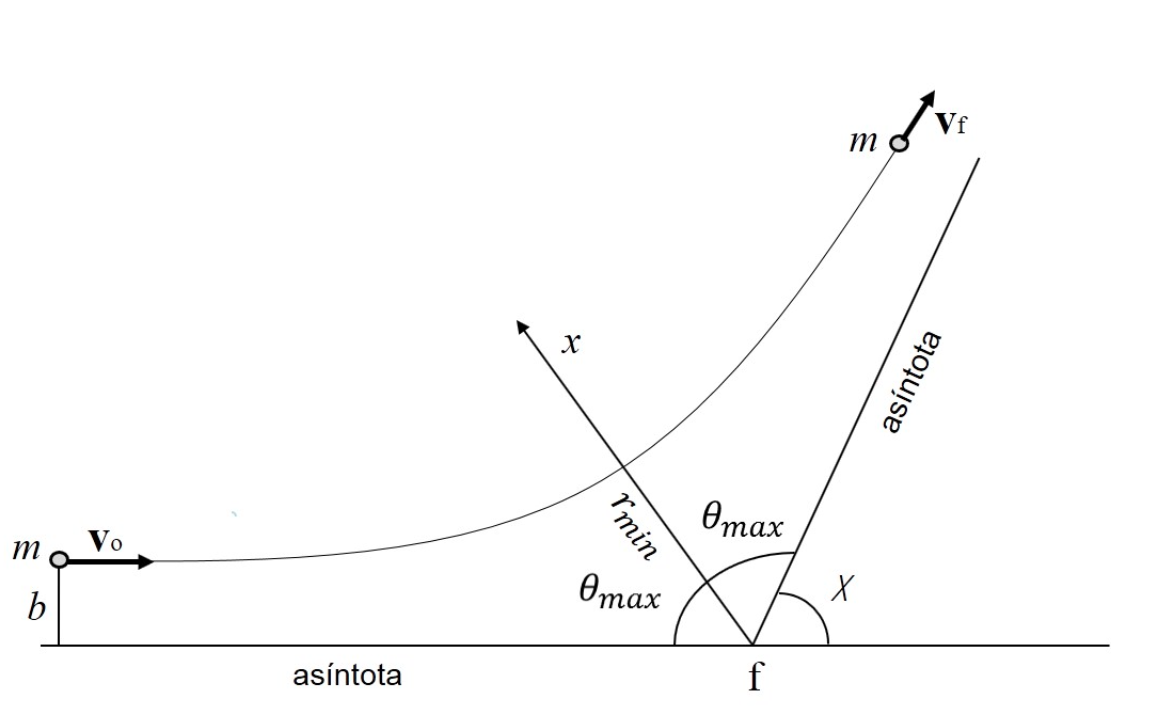
\includegraphics[width=1.8in]{Figuras/Dispersion.png}
   	\end{figure}
	
